\documentclass[a4paper]{article}

	%% Language and font encodings
	\usepackage[english,spanish]{babel}
	\usepackage[utf8x]{inputenc}
	\usepackage[T1]{fontenc}
	
	\usepackage{hyperref}
	\usepackage{caption}
	\usepackage{subcaption}
	\usepackage{booktabs}
	
	%% Sets page size and margins
	\usepackage[a4paper,top=3cm,bottom=2cm,left=3cm,right=3cm,marginparwidth=1.75cm]{geometry}
	
	%% Useful packages
	\usepackage{amsmath}
	\usepackage{graphicx}
	\usepackage[colorinlistoftodos]{todonotes}
	
	\begin{document}
	
	\title{%
	% \includegraphics[scale = 0.5]{./header_unc.png}\\[1.0 cm]	% University Logo
	  Arquitectura de Computadoras \\
	  \large Ingeniería en Computación FCEFyN - UNC\\
			  Simulador Tomasulo con ROB
	  }
	
	
	  \author{Aguerreberry Matthew. Mat.: 93739112}
	  
	  \maketitle
	  
	  \section{Introducción}
	  
	  Se busca implementar un simulador en Python del algoritmo de Tomasulo con Buffer de reordenamiento.
	  
	  \begin{figure}[!h]
	  \centering
	  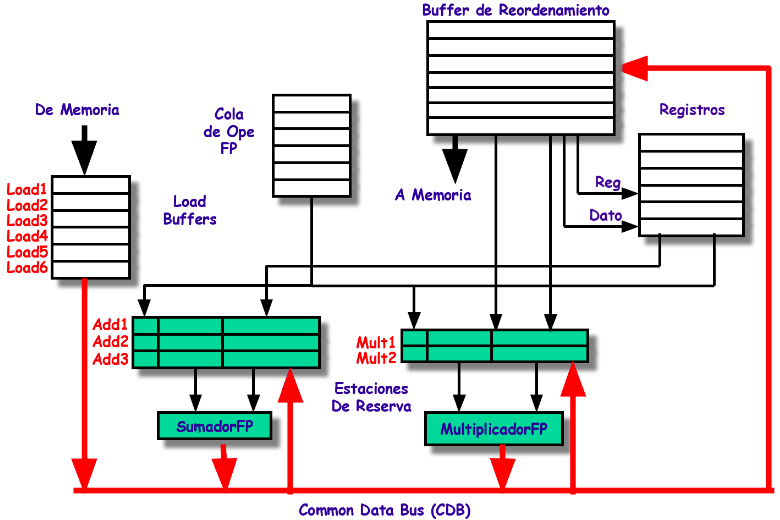
\includegraphics[width=.7\textwidth]{figures/esquema.png}
	  \caption{\label{fig:bloques}Esquema del algoritmo de Tomasulo con ROB}
	  \end{figure}

		
	\subsection{Supuestos}
	
	  Los supuesto a priori y restricciones de la implementación son:

	  \begin{itemize}
		  \item Se cuenta con tres unidades de ejecución. Un sumador para operaciones enteras, un sumador para operaciones de punto flotante y un multiplicador para operaciones de punto flotante.
		  \item La duración de la unidades de ejecución son:
		  \begin{itemize}
			  \item Sumador entero: 1 ciclo. Con 2 estaciones de reserva.
			  \item Sumador punto flotante: 4 ciclos. Con 3 estaciones de reserva.
			  \item Multiplicador punto flotante: 8 ciclos. Con 2 estaciones de reserva.
			  \item Memoria: 4 ciclos. Con 3 entradas en el buffer de load-store.
		  \end{itemize}
	  \end{itemize}

	\section{Diagramas UML}

	\subsection*{Estados}
	\subsection*{Clases}
	\subsection*{Secuencia}
	
	\section{Verificación y Validación}

	

	\section{Conclusiones}
	
	

	\end{document}